%%%%%%%%%%%%%%%%%%%%%%%%%%%%%%%%%%%%%%%%%
% University Assignment Title Page 
% LaTeX Template
% Version 1.0 (27/12/12)
%
% This template has been downloaded from:
% http://www.LaTeXTemplates.com
%
% Original author:
% WikiBooks (http://en.wikibooks.org/wiki/LaTeX/Title_Creation)
%
% License:
% CC BY-NC-SA 3.0 (http://creativecommons.org/licenses/by-nc-sa/3.0/)
% 
% Instructions for using this template:
% This title page is capable of being compiled as is. This is not useful for 
% including it in another document. To do this, you have two options: 
%
% 1) Copy/paste everything between \begin{document} and \end{document} 
% starting at \begin{titlepage} and paste this into another LaTeX file where you 
% want your title page.
% OR
% 2) Remove everything outside the \begin{titlepage} and \end{titlepage} and 
% move this file to the same directory as the LaTeX file you wish to add it to. 
% Then add \input{./title_page_1.tex} to your LaTeX file where you want your
% title page.
%
%%%%%%%%%%%%%%%%%%%%%%%%%%%%%%%%%%%%%%%%%
%\title{Title page with logo}
%----------------------------------------------------------------------------------------
%	PACKAGES AND OTHER DOCUMENT CONFIGURATIONS
%----------------------------------------------------------------------------------------

\documentclass[12pt, table,xcdraw]{article}
\usepackage[english]{babel}
\usepackage[utf8x]{inputenc}
\usepackage{amsmath}
\usepackage{graphicx}
\usepackage{multirow}
%\usepackage[table,xcdraw]{xcolor}
\usepackage[colorinlistoftodos]{todonotes}
\usepackage{bigstrut}
\usepackage{subfigure}
\usepackage{caption} 
\captionsetup[table]{skip=6pt}



\begin{document}

\begin{titlepage}

\newcommand{\HRule}{\rule{\linewidth}{0.5mm}} % Defines a new command for the horizontal lines, change thickness here

\center % Center everything on the page
 
%----------------------------------------------------------------------------------------
%	HEADING SECTIONS
%----------------------------------------------------------------------------------------

\textsc{\LARGE Università degli studi di Milano-Bicocca}\\[1cm] % Name of your university/college
\textsc{\Large Advanced Machine Learning }\\[0.3cm] % Major heading such as course name
\textsc{\large Final Project}\\[0.1cm] % Minor heading such as course title

%----------------------------------------------------------------------------------------
%	TITLE SECTION
%----------------------------------------------------------------------------------------

\HRule \\[0.4cm]
{ \huge \bfseries Classification of flower images starting from a small dataset}\\[0.4cm] % Title of your document
\HRule \\[1.5cm]
 
%----------------------------------------------------------------------------------------
%	AUTHOR SECTION
%----------------------------------------------------------------------------------------

\large
\emph{Author:}\\
David Bertoldi - 735213 - d.bertoldi@campus.unimib.it \\[1cm]  % Your name


% If you don't want a supervisor, uncomment the two lines below and remove the section above
%\Large \emph{Author:}\\
%John \textsc{Smith}\\[3cm] % Your name

%----------------------------------------------------------------------------------------
%	DATE SECTION
%----------------------------------------------------------------------------------------

{\large \today}\\[2cm] % Date, change the \today to a set date if you want to be precise

%----------------------------------------------------------------------------------------
%	LOGO SECTION
%----------------------------------------------------------------------------------------


\includegraphics{logo.png}\\[1cm] % Include a department/university logo - this will require the graphicx package
 
%----------------------------------------------------------------------------------------

\vfill % Fill the rest of the page with whitespace

\end{titlepage}


\begin{abstract}
This work describes a supervised approach to classification of images on a small dataset, but with a large number of classes. In particular, it is shown how the
combination of modern training techniques and recent developments
in the field of research of architectures for neural networks are able
to obtain high performances even when the model is partially trained.
\end{abstract}

\section{Introduction}


The aim of this work is to build a machine learning model able to learn from a small knowledge base and to classify similar images but belonging to different classes.
The main issue to overcome was the high chance that the model could overfit and fail to classify unseen samples. 
The strategy adopted was to find the model exploiting transfer learning the best and then trying to freeze the model such that it could maintain similar performances. \par
This document describes the research on trained models, hyperparameters and generalization techniques that allowed the model to operate on a large variety of images. 






\section{Datasets}
The dataset used is the \textit{102 Category Flower Dataset} \cite{Nilsback08} created by the researchers of the \textit{Visual Geometry Group} of \textit{Oxford}. The dataset is composed of $8189$ RGB images of variable size, each image contains one or more flowers on a neutral background and is labeled with a single category extracted from a set of $102$ possible categories. The original dataset also contains the flowers segmented from the background (Figure \ref{fig_dataset}); these images can be used for example as further input for the neural network. In this work they were not used in order to force the model to be more elastic with respect to the background of the images. \par
The subdivision of the dataset defined in the original publication has been maintained, in particular there are $1020$ images in the training set, $1020$ images in the validation set and $6149$ images in the test set.

\begin{figure}[ht!]
\centering  
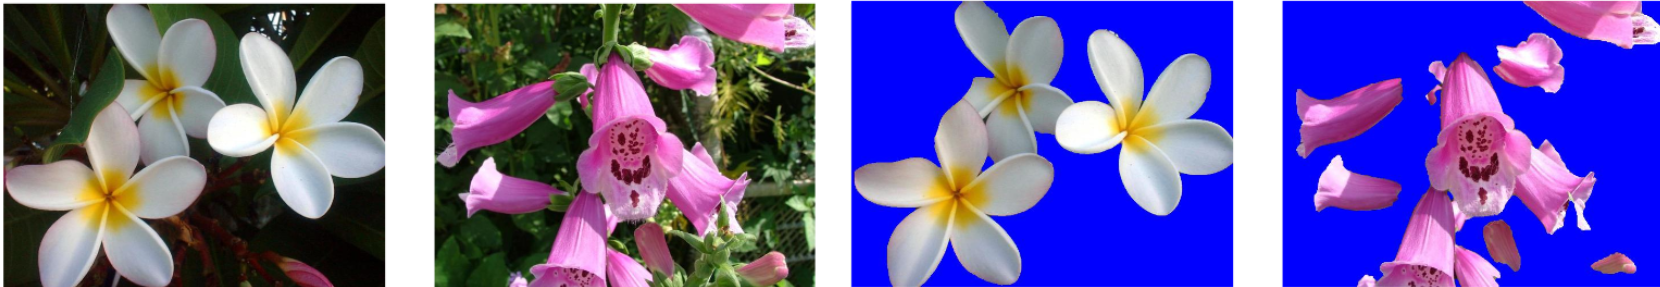
\includegraphics[width=1.0\textwidth]{images/dataset.png} 
\caption{Training images and their segmentation}
\label{fig_dataset}
\end{figure}

Each category is represented by $10$ images in the training set and validation set, while the proportion of images for each category varies in the test set. Figure \ref{fig:dist} plots the distribution of the three datasets: the distribution of the samples is non-uniform across the categories, with a mean $\mu \simeq 60$ and standard deviation $\sigma \simeq 44$. In fact some classes had more than 200 samples, like  $50$ (\textit{Common Dandelion}) and $78$ (\textit{Lotus}) and other just $20$ per class, like $1$ (\textit{Pink Primrose}), $17$ (\textit{Purple Coneflower}) or $23$ (\textit{Fritillary}).

\begin{figure}[ht!]
\centering
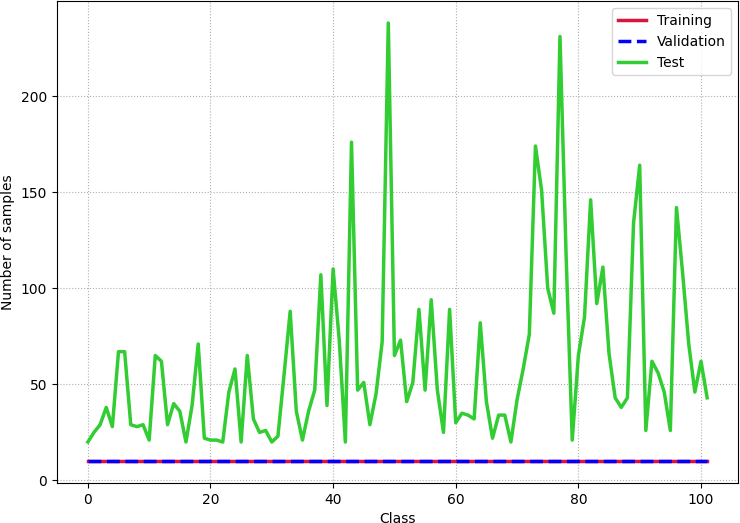
\includegraphics[width=0.8\textwidth]{images/dist.png} 
\caption{Distribution of the samples for each category in each dataset}
\label{fig:dist}
\end{figure}

The difficulty of operating on a dataset of this type is evident: the number of images for training is limited while the test set is larger. 

\par
Another peculiarity of the dataset is the presence of similar images belonging to different categories.



















\section{The Methodological Approach}

Two experiments are proposed in this work: the first one aimed to find the best CNN\footnote{Convolutional Neural Network} architectures in 
literature that could fit the available hardware (see Section \ref{sec:tech}) and fine-tuned it in order to classify images correctly; the objective of the second one was to find a good trade-off between number of trainable layers, training time and accuracy by freezing the layers' weights during training so that the training on new classes could be faster. \par

All the proposed architectures were pre-trained on \textit{ImageNet}\cite{5206848} and used as feature extractors for a new classifier that operates over 102 classes (see Section \ref{sec:exp1} for details about the architecture).

\subsection{Technology and implementation}\label{sec:tech}
The hardware used for this work was composed by a GPU NVIDIA 2070 SUPER with 8GB of VRAM, a CPU Intel i7-9700K $3.6$GHz and $32$GB of RAM. \par
The libraries used were \textit{Keras}, based on \textit{Tensorflow}, for learning and preprocessing, \textit{sklearn} for metrics and \textit{numpy}  for generic calculations.


\subsection{Data Augmentation and Preprocessing}
Before proceeding with the description of the experiments, there was a preliminar implicit objective: a way to overcome the scarcity of training data.\par
In order to raise the number of samples it was used \texttt{ImageDataGenerator}\footnote{Although it is deprecated, the API is easy to use and already optimized. The suggested way with \texttt{tf.keras.utils.image\_dataset\_from\_directory} and \texttt{tf.data.Dataset} is more flexible, but harder to optimize properly. \texttt{ImageDataGenerator} API was preferable in terms of development speed.} from \textit{Keras}. This allowed to virtually loop infinitely on the images during the training and most importantly to transform each of these images by applying none, one or more of the following transformations:
\begin{itemize}
\item{Horizontal flipping}
\item{Rotation of angle $\alpha \in [-20^{\circ}, 20^{\circ}]$}
\item{Shift of brightness $\gamma \in [0.7, 1.3]$}
\item{Zoom  $\zeta \in [0.8, 1.2]$}
\end{itemize}
Additionally every image is transformed with the original preprocessing function used for the training of the original architecture on \textit{ImageNet}. In Sections \ref{sec:resnet18}, \ref{sec:inceptionv3} and \ref{sec:efficientnetb4} there are more details about it.


\subsection{Hyper-parameters}
To train the classifier on the extracted features it was decided to use the SGD \cite{kiefer1952} with momentum $\beta = 0.9$ or Adam \cite{kingma2014adam} with $\beta_1 = 0.9$ and $\beta_2 = 0.999$, with dimension of
batch equal to $64$.
Since the task is a classification over multiple categories the chosen objective function to minimize was \emph{categorical cross-entropy}. \par

The learning rate $\eta$ is calculated according to the algorithm described in \emph{"Cyclical Learning Rates for Training Neural
Networks”} \cite{smith2015cyclical}. This algorithm made $\eta$ fluctuate forward and
back in a fixed interval $I$ at each iteration during the training phase;
this strategy had a dual purpose: to reduce the bias introduced by choosing a non-optimal $\eta$ during the design phase and to help the optimizer to escape from saddle points or 
from local minima that could block its correct covergence.\par

To calculate the aforementioned interval $I$ of values the authors described the \textit{Learning Rate Finder} algorithm (LRF):
\begin{enumerate}
\item{Choose an interval $J$ on which to make vary $\eta$. For this work $J = [10^{-10}, 10^{-1}]$ was used} 
\item{Train the model for few epochs (\textit{e.g.} 10) starting with the smallest ${\eta}' \in J$. At the end of each epoch exponentially increase ${\eta}'$}
\item{Stop the training when ${\eta}'$ reached the upper bound of $J$}
\item{Plot the fluctuation of the loss function realtive to ${\eta}'$}
\end{enumerate}
As an example, the algorithm generated the plot in Figure \ref{fig:lr} for optimizer Adam and the architecture described in section \ref{sec:resnet18}. 
\begin{figure}[ht]
\centering
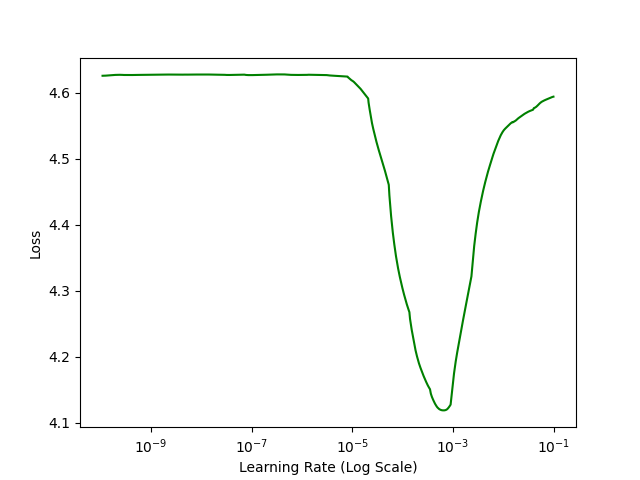
\includegraphics[width=0.7\textwidth]{images/lr_adam.png} 
\caption{Output of the learning rate finder algorithm. $I=[10^{-5}, 10^{-3}]$ is the optimal solution}
\label{fig:lr}
\end{figure}

The graph shows how the network begins to learn starting from $\eta \simeq 10^{-5}$ and diverges once $\eta$ exceeded $\sim10^{-3}$; these two values were used as extremes of $I$ for the cyclical learning rate algorithm on this particular architecture.\par
The drawback of this strategy is that it added two additional hyper-parameters: the step size $s$, that determined the number of iterations required to go from the minimum $\eta \in I$ to the maximum, and the cyclical learning rate schedule, that defined the way $\eta$ is modified. \par

Figure \ref{fig:triangular} shows the two schedules used for this work: \emph{Triangular} and \emph{Triangular2};
the difference between the two is that the second method halves the upper bound of $I$ at each cycle completion.
\begin{figure}[ht!]
\centering
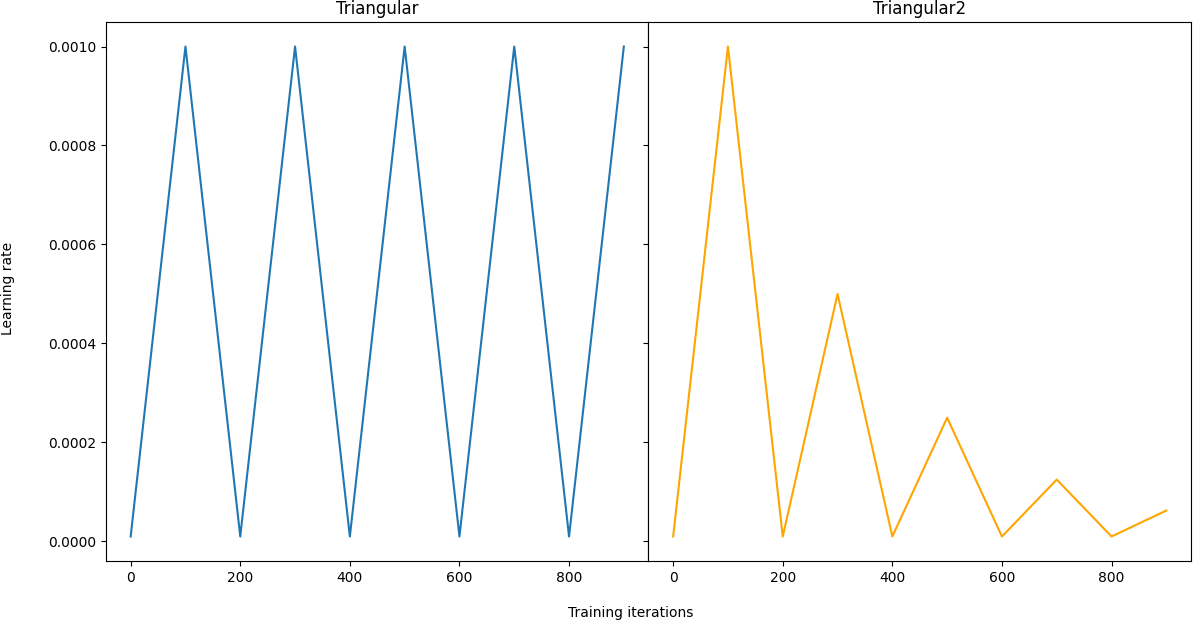
\includegraphics[width=0.8\textwidth]{images/triangular.png} 
\caption{Plot of the learning rate with \emph{Triangular} and \emph{Triangular2} methods}
\label{fig:triangular}
\end{figure}








\subsection{Experiment 1: Choice of the architecture}\label{sec:exp1}
The first experiment aimed to find the architecture that could achieve the best accuracy on the test set. This work tested \textit{ResNet-18} \cite{he2015deep}, \textit{InceptionV3} \cite{szegedy2015going} and 
\textit{EfficientNetB4} \cite{tan2019efficientnet}. All of them presented diffent peculiarities and could be used for training with the available hardware. \par
Since the training on \textit{ImageNet} of the networks is not sufficient to use them as feature extractors, these networks were fine-tuned in order to update their weights and to fit better the task.\par
\begin{figure}[ht!]
\centering
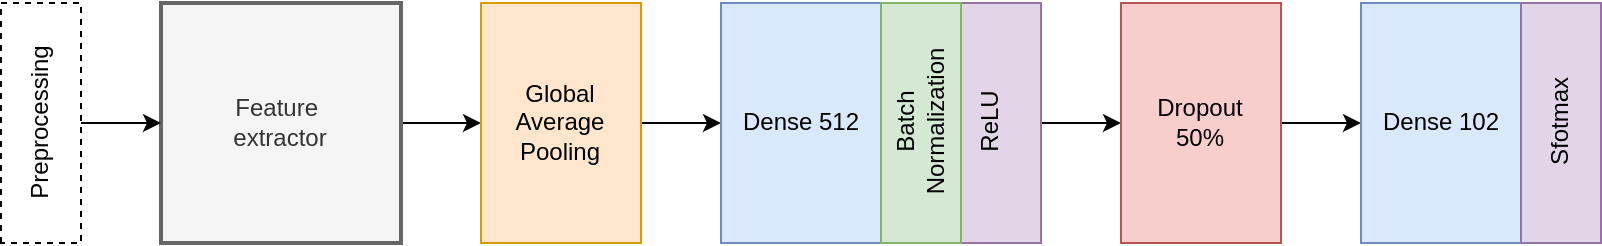
\includegraphics[width=1\textwidth]{images/architecture.png} 
\caption{High level architecture of the network: in grey the pretrained network used as feature extractor, followed by the classifier's layers.}
\label{fig:architecture}
\end{figure}




For each networks the original classification layers were removed and substituted with a new classifier composed by the following layers:
\begin{enumerate}
\item{\textbf{Global Average Pooling}: instead of using a Flatten layer that could raise the risk of overfitting and forced the use of Dropout, this layer applied average pooling on the spatial dimensions until each spatial dimension is one, and leaves other dimensions unchanged. It added 0 new parameters to the model} 
\item{\textbf{Dense 512}: a dense layer with a \textbf{Batch Normalization} before the activation function (ReLU). This helped to avoid vanishing/exploding gradients when training the model. It added $512 \cdot (n+1) + 4\cdot512 = 512n + 2560$ parameters}
\item{\textbf{Dropout} as regularization technique for reducing overfitting during training, with a drop rate $\rho=0.5$. It added 0 new parameters to the model}
\item{\textbf{Dense 102}: a dense layer that used softmax as activation function. It added  $102 \cdot (512+1) = 52326$ new parameters}
\end{enumerate}
Figure \ref{fig:architecture} gives an overview of the architecture described above.
The total number of parameters added to the original feature extractor is $512n + 54886$, where $n$ is the dimensionality of the last layer of the feature extractor.\par
The strategy adopted for training is the same for all the three networks: each network is trained with 3 different step sizes $s \in \{2,4,8\}$, two different optimizers (\textit{SGD} and \textit{Adam}) and 2 different learning rate schedulers (\emph{Triangular} and \emph{Triangular2}). So each network is trained 12 times in order to find the best configuration. For this phase it was implemented the \textit{Early Stopping} technique in order to prevent overfitting and to speed up the training by stopping prematurely the process. This strategy monitored the validation accuracy and stopped everytime a model could not improve by $0.5\%$ in the last $10$ epochs.



\subsubsection{Fine-tuning of ResNet-18}\label{sec:resnet18}
ResNet-18 is a convolutional neural network that is 18 layers deep and accepts images of input size of $224 \times 224$. It is a residual network, that is it implements skip connections to help to address the problem of vanishing  gradients. \par
The preprocessing function applied on the images converted them from RGB to BGR, then each color channel was zero-centered with respect to the \textit{ImageNet} dataset, without scaling. \par
From the output of the \textit{LRF} algorithm the learning rate was varied in the interval $[10^{-6}, 10^{-4}]$ for SGD and $[10^{-5}, 10^{-3}]$ for Adam.


\subsubsection{Fine-tuning of InceptionV3}\label{sec:inceptionv3}
InceptionV3 is a convolutional neural network that is 42 layers deep and accepts images of input size of $299 \times 299$. This architecture factorizes the larger convolutions  into smaller ones and and uses an auxiliary classifer to propagate label information lower down the network.
 \par
The preprocessing function applied on the images scaled their pixels between -1 and 1, sample-wise. \par
From the output of the \textit{LRF} algorithm the learning rate was varied in the interval $[10^{-5}, 10^{-2}]$ for SGD and $[10^{-4}, 10^{-2}]$ for Adam.


\subsubsection{Fine-tuning of EfficientNetB4}\label{sec:efficientnetb4}
EfficientNetB4 is a convolutional neural network that is 237 layers deep and accepts images of input size of $224 \times 224$. 
This type of architecture was built using automatic search and scaling techniques
aimed to simultaneously maximize the accuracy of the network and the number of operations per second. \par
There was no need to apply the ad-hoc preprocessing function because it was embedded in the \textit{Keras} implementation. \par
From the output of the \textit{LRF} algorithm the learning rate was varied in the interval $[10^{-5}, 10^{-3}]$ fboth or \textit{SGD} and \textit{Adam}.


\subsection{Evaluation of the training}
To verify the quality of the training two techniques were applied: \textit{grad-CAM} \cite{Selvaraju_2019}  and \textit{Saliency Map} \cite{simonyan2013deep}. Confusion matrices \cite{Stehman1997} as well helped indentifying
issues in the first stages of the implementation.

\subsubsection{grad-CAM}
\textit{grad-CAM} uses the gradient of the last convolutional layer so that the spatial information are preserved. An heatmap is displayed over the original image
that shows the main component identified by the network.

\begin{figure}[ht!]
\centering
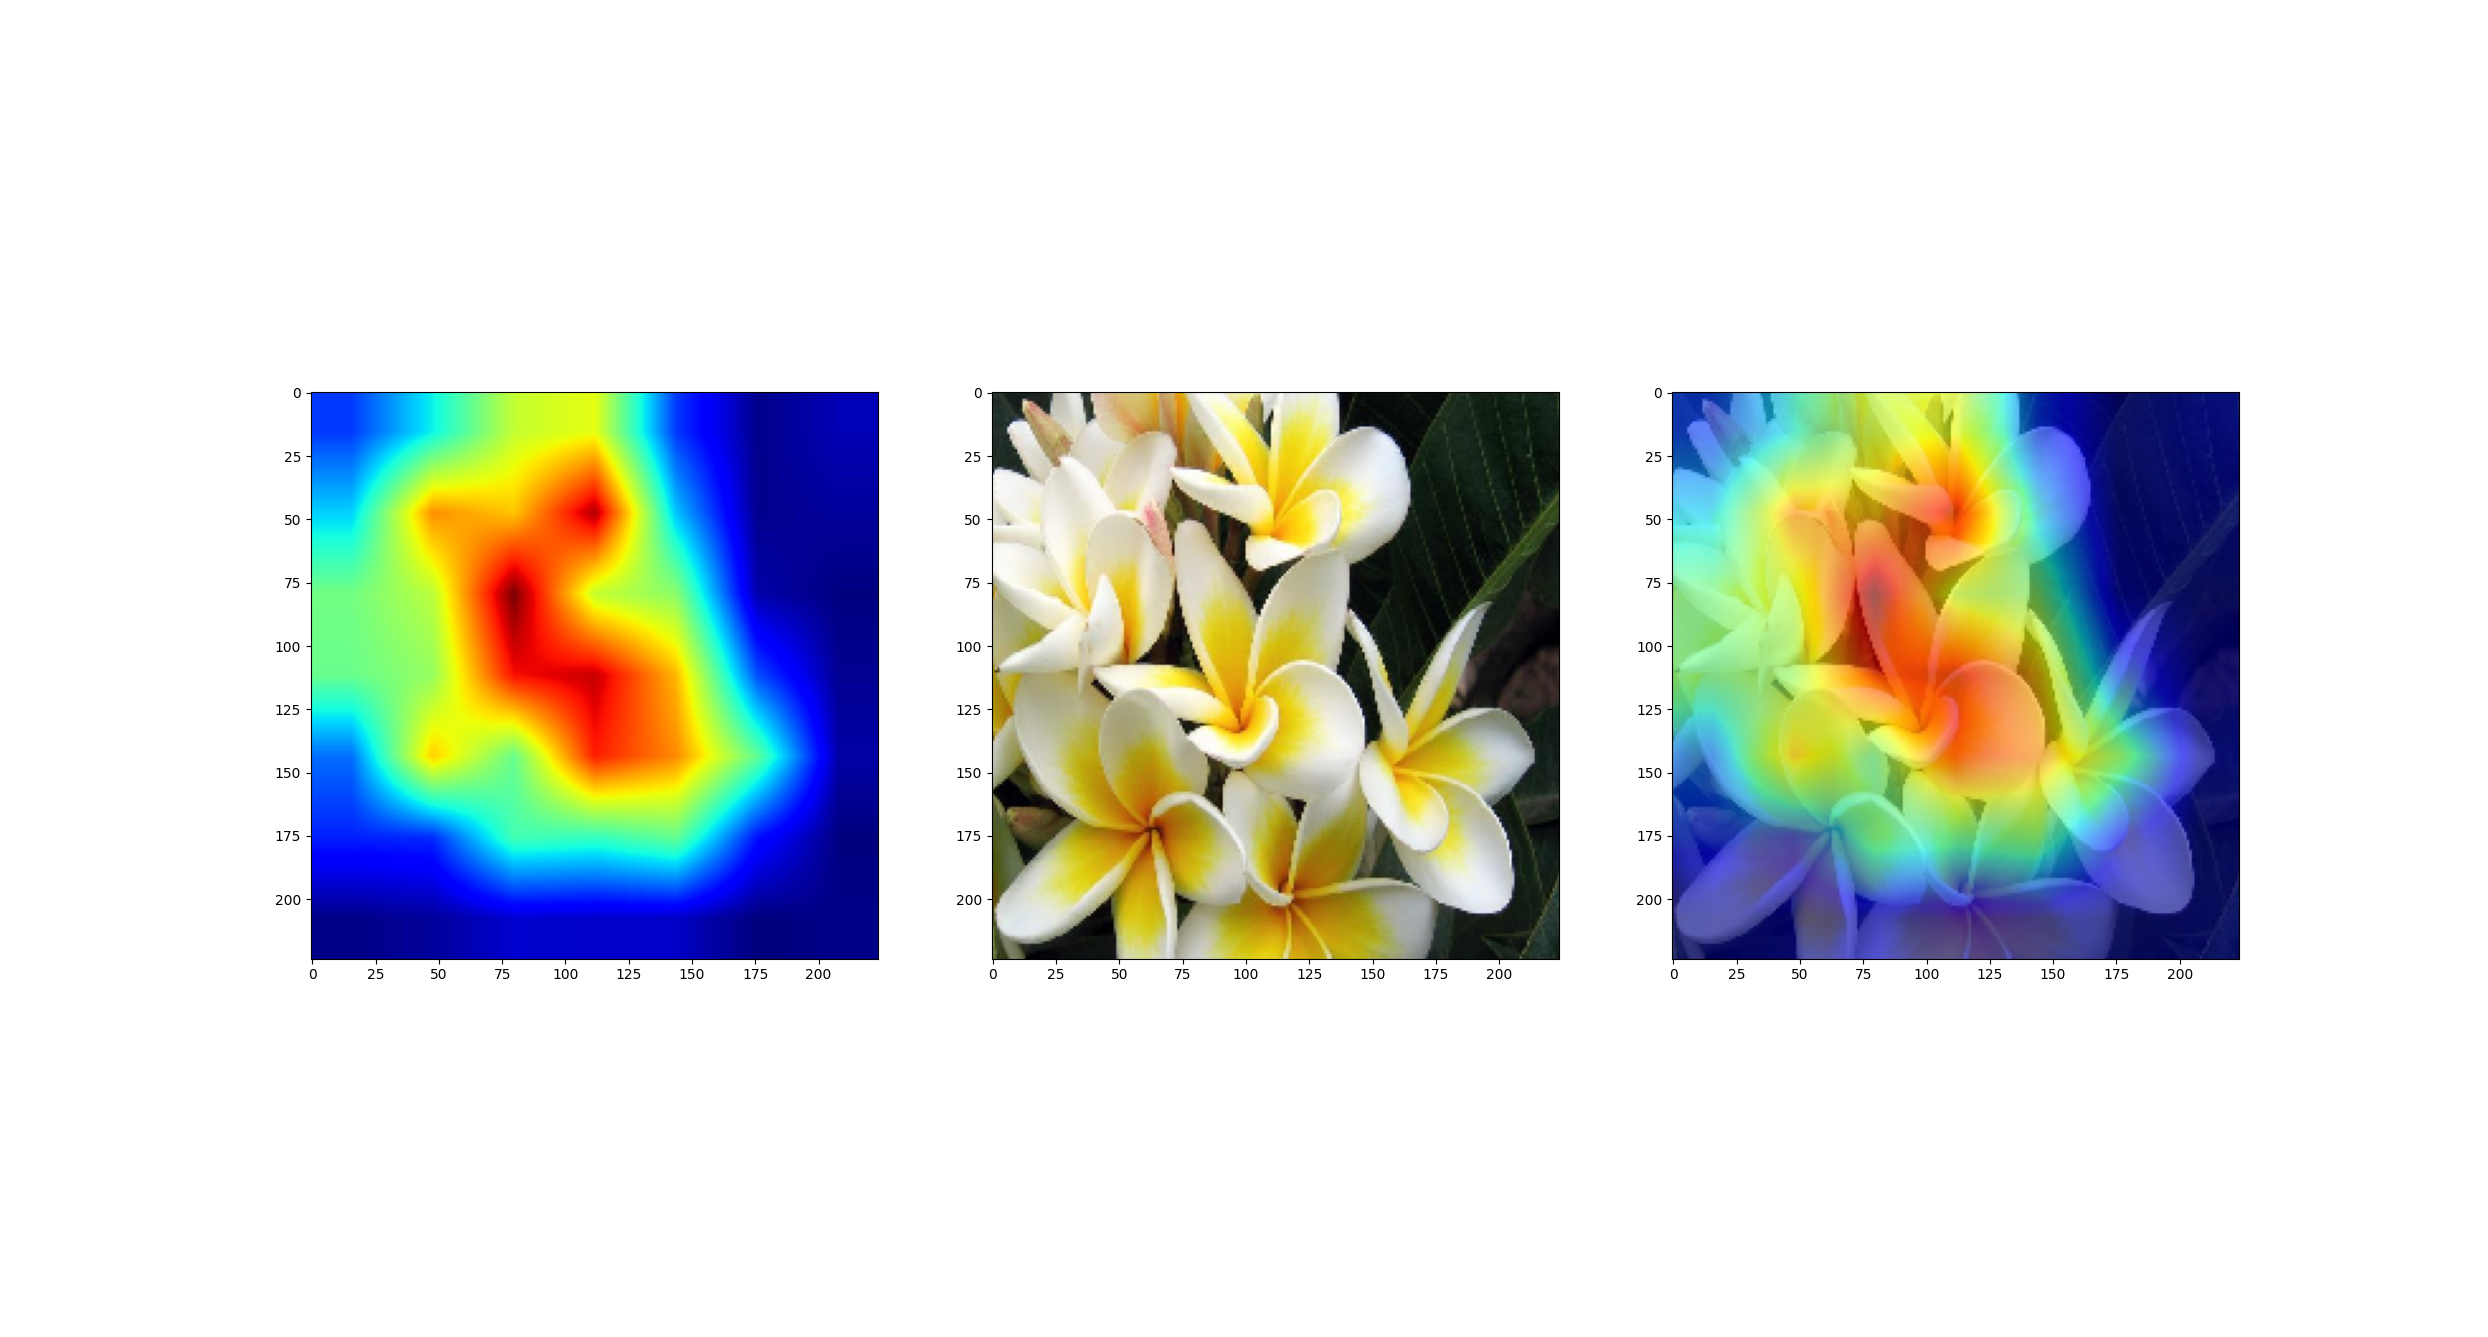
\includegraphics[width=1\textwidth]{images/grad_multi.png} 
\caption{\textit{grad-CAM} of multiple flowers extracted from EfficientNetB4}
\label{fig:grad_multi}
\end{figure}

For example Figure \ref{fig:grad_multi} demonstrates that the model could distinguish multiple flowers from the background and that the background is not an important 
feature to be learned.


\subsubsection{Saliency Map}
Like the \textit{grad-CAM}, \textit{Saliency Maps} analyze a specific layer of the model, but in this case it is a classification layer. It shows the gradients of
an image with respect with the label. The map indicates the points that affected more the correct classification of the image.
\begin{figure}[ht!]
\centering
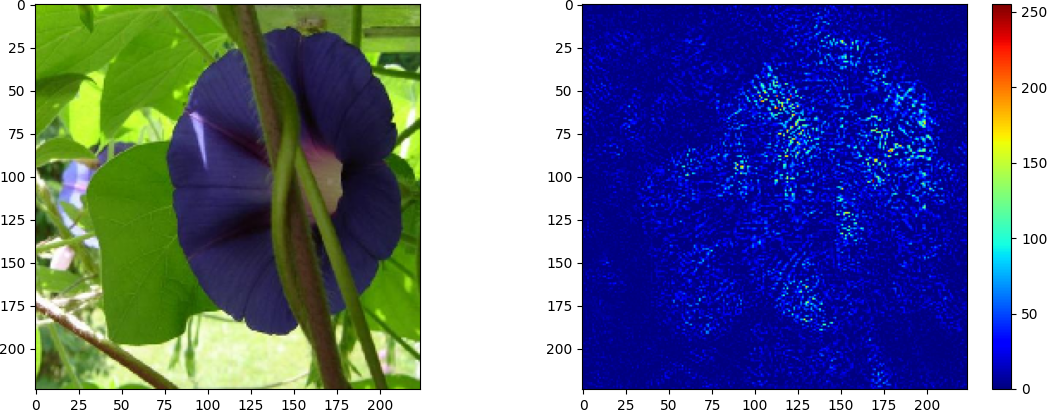
\includegraphics[width=1\textwidth]{images/sal3.png} 
\caption{Example of \textit{Saliency Map} extracted from EfficientNetB4 of a flower with an obstacle in front of it}
\label{fig:sal}
\end{figure}

As can be seen in figure \ref{fig:sal} most of the pixels that affect the
classification is contained within the flower and this is a good indicator
of the quality of the model.







\subsection{Experiment 2: Freeze layers}\label{sec:exp2}
The aim of this second experiment was to find an architecture derived from the first experiment that could be trained again or trained with new classes\footnote{Not provided by the original dataset.} with better timings but preserving accuracy as much as possible.
This means that the objective was to find a good trade-off between the number of trainable parameters, test accuracy and training time: after choosing the best model from Section \ref{sec:exp1}, its layers were frozen so that the weight would not be updated during training. The layers were frozen starting from the input to the deeper layers and because the training dataset is small and different from \textit{ImageNet} dataset it was expected to have better performances when only a small portion of layers is locked. Only the feature extractor was affected by this process, while the classificator reamined fully trainable. This allowed to freeze from $10\%$ to $100\%$ of the feature extractor's layers.\par
In order to have an accurate estimation of the timings the \textit{Early Stopping} strategy was disabled because it could terminate prematurely the training process. This limitation afflicted the accuracy because the model could have overfitted more than the regularized version.
\par
The results were evaluated considering, in order of importance,  the accuracy on the test dataset, the training time and the number of trainable parameters. 





\section{Results and Evaluation}
This section reports the results obtained for both the experiments. 


\subsection{Experiment 1}

Table \ref{tab:res} shows the configuration that gave the best results for
 each architecture. Figure \ref{fig:cm} shows the confusion matrix on the test set for EfficientNetB4.

\begin{table}[ht!]
\centering
\caption{}
\label{tab:res}
\resizebox{\columnwidth}{!}{%
\begin{tabular}{|l|l|l|l|l|l|l|}
\hline
\textbf{Archtecture} & \textbf{Batch size} & \textbf{Optimizer} & \textbf{Learning rate} & \textbf{Scheduler} & \textbf{Step size} & \textbf{Test accuracy} \\ \hline
ResNet-18      & 64 & Adam & $[10^{-5}, 10^{-3}]$ & Triangular  & 2 & 87.64\% \\ \hline
InceptionV3    & 64 & Adam & $[10^{-4}, 10^{-2}]$ & Triangular  & 2 & 91.96\% \\ \hline
EfficientNetB4 & 16 & Adam & $[10^{-5}, 10^{-3}]$ & Triangualr2 & 4 & 94.89\% \\ \hline
\end{tabular}%
}
\end{table}

Appendix \ref{sec:app} shows in tabular form all the results from the 12 trainings of each model.

\begin{figure}[ht!]
\centering
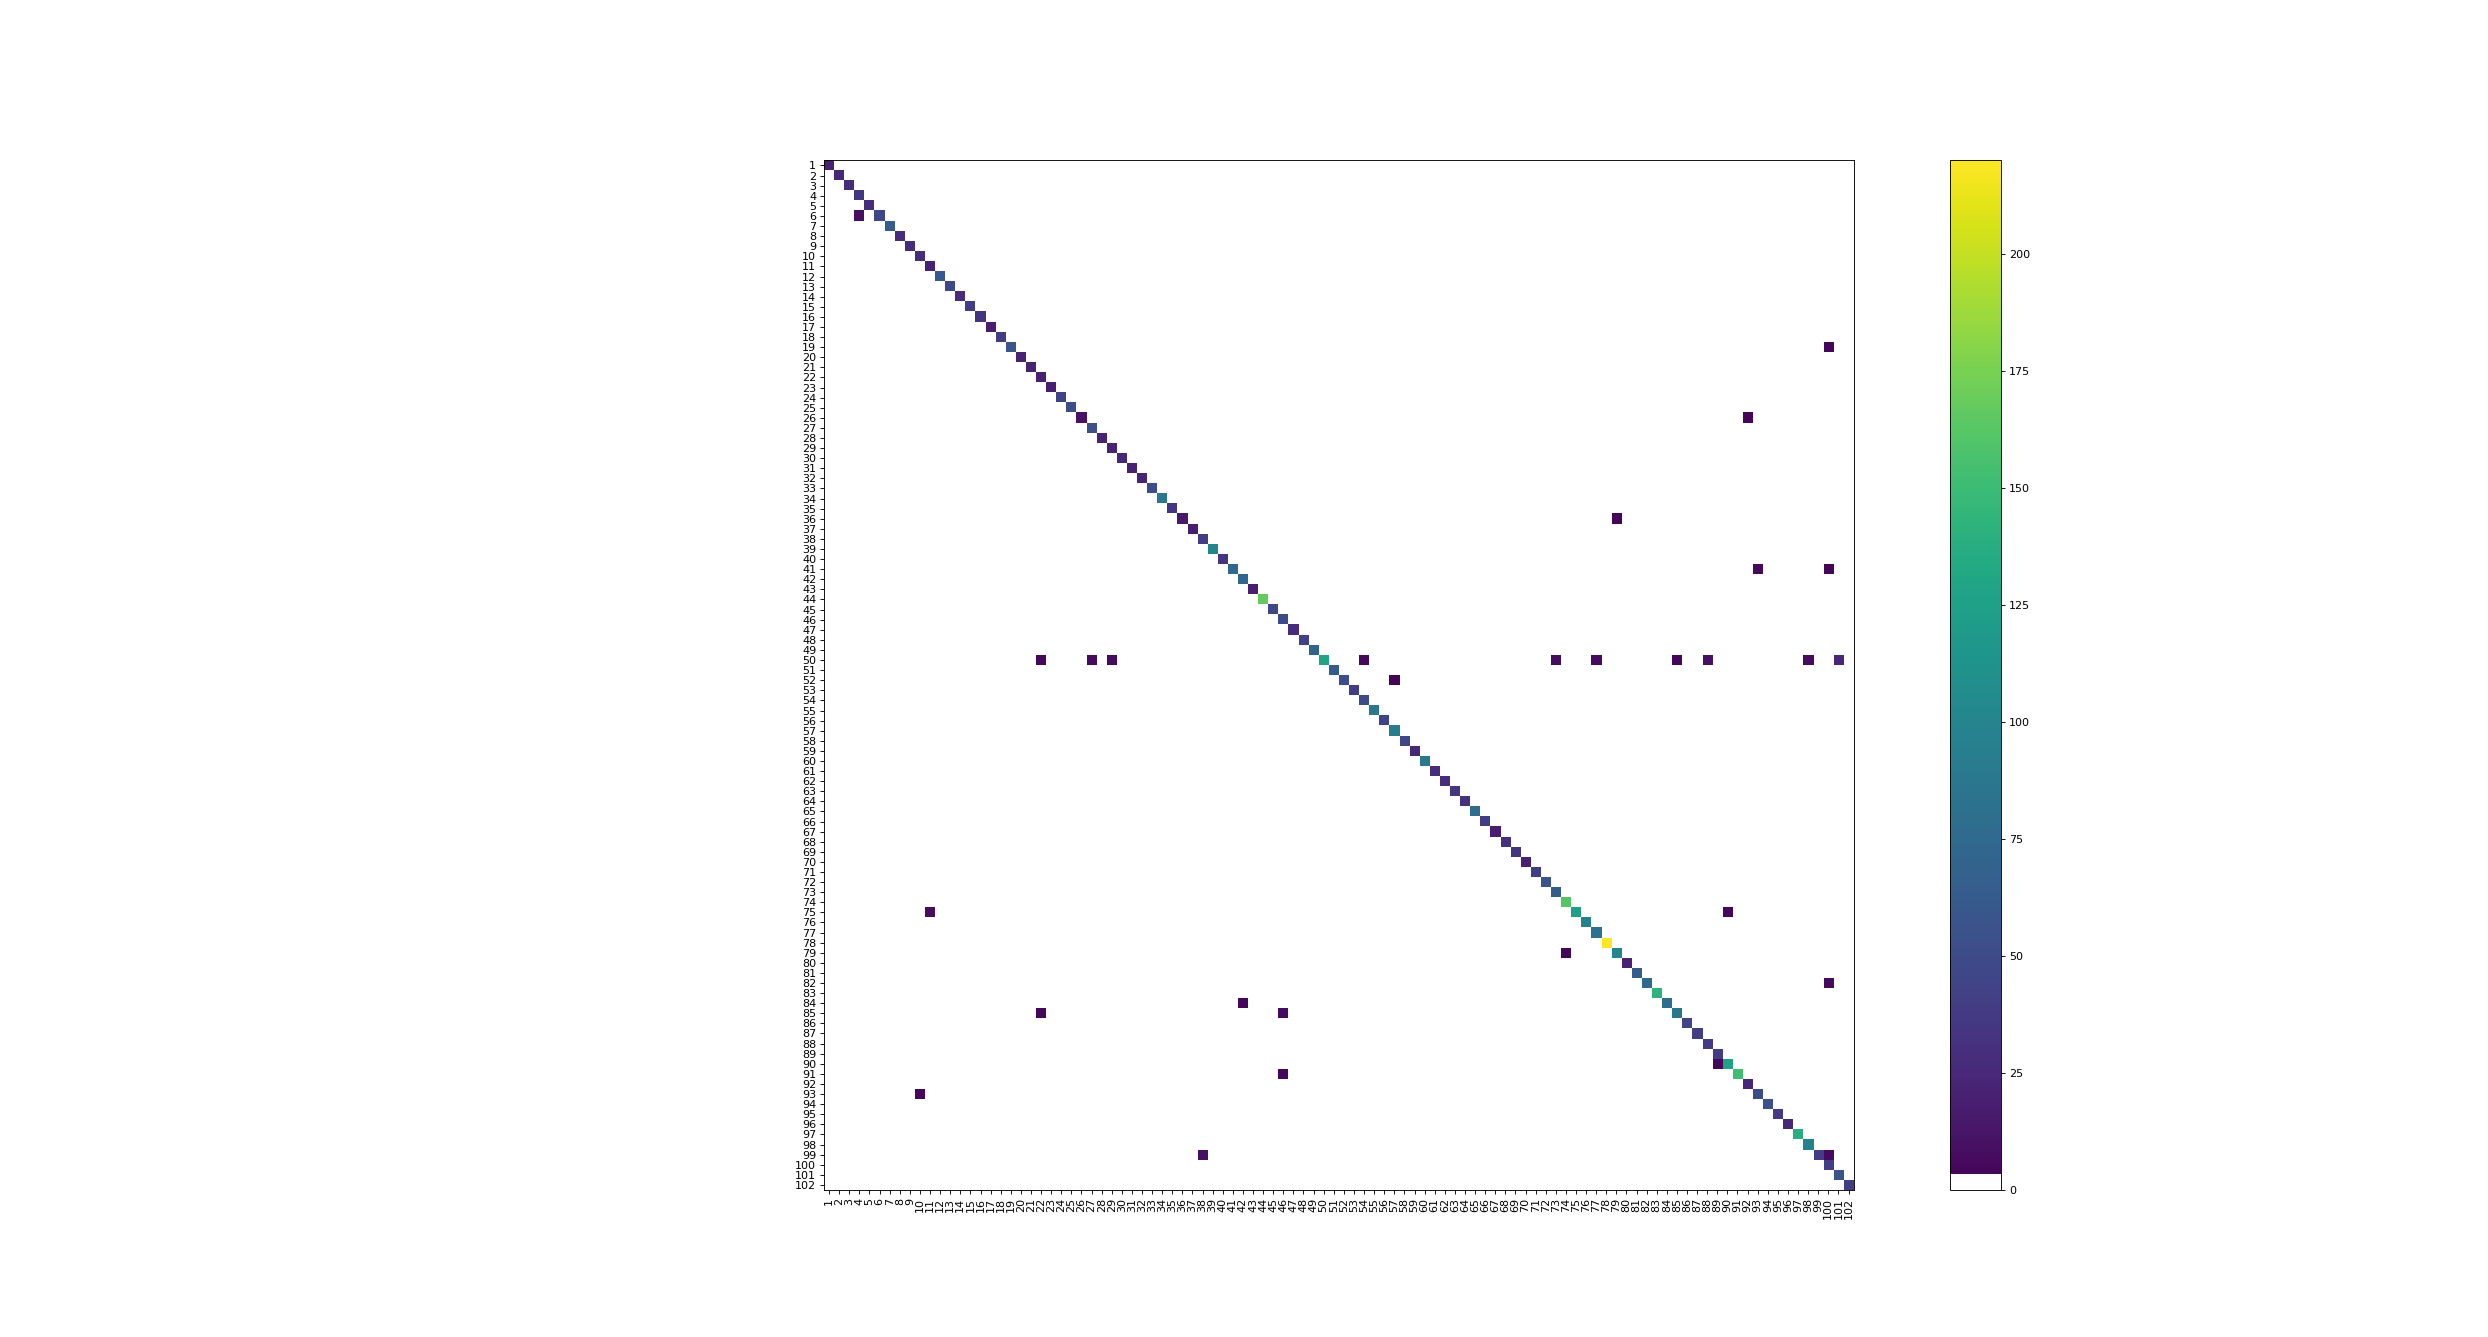
\includegraphics[width=1\textwidth]{images/cm.png} 
\caption{Confusion matrix of EfficientNetB4 on the test dataset}
\label{fig:cm}
\end{figure}

\subsection{Experiment 2}\label{sec:exp2}


It is immediately noticeable that EfficientNetB4 from the first experiment performed better than the other models and for this reason it was chosen for the second experiment. Figure \ref{fig:time_acc}a compares the accuracy on the test dataset and the number of trainable parameters as the number of frozen layers increased. Figure \ref{fig:time_acc}b compares accuracy and training time with respect to the number of frozen layers. Table \ref{tab:frozen} shows the data in tabular form.


\begin{figure}
    \centering
    \subfigure[]{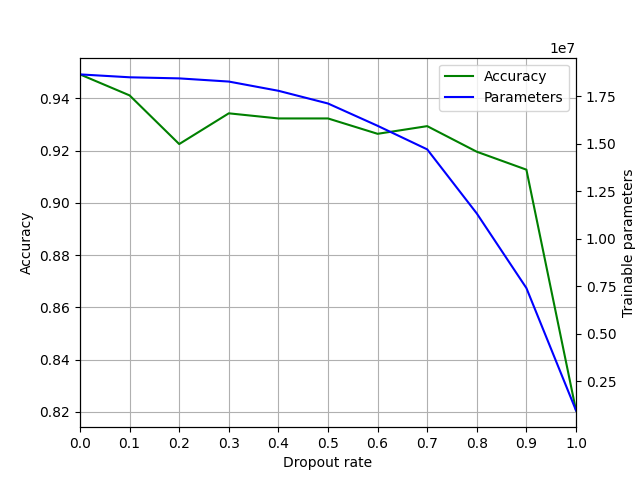
\includegraphics[width=0.48\textwidth]{images/param_acc.png}} 
    \subfigure[]{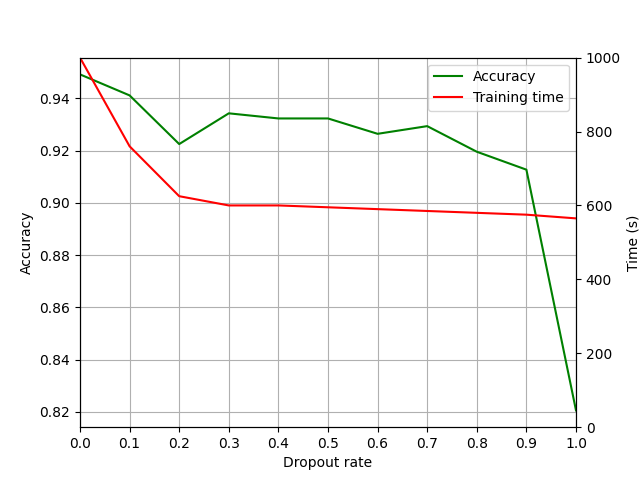
\includegraphics[width=0.48\textwidth]{images/time_acc.png}} 
    \caption{Plot of the accuracy compared to the number of trainable parameters (a) and compared to training time (b) as the number of frozen layers varies}
    \label{fig:time_acc}
\end{figure}

\begin{table}[ht!]
\centering
\caption{\textit{EfficientNetB4}: Comparisong between accuracy, trainable parameters and training time as the number of frozen layers increased }
\label{tab:frozen}
\resizebox{\columnwidth}{!}{%
\begin{tabular}{|l|l|l|l|}
\hline
\textbf{Freeze Rate} & \textbf{Trainable Parameters} & \textbf{Accuracy} & \textbf{Training Time} \\ \hline
10\%                 & 18,494,310                    & 94.11\%           & 760s                   \\ \hline
20\%                 & 18,436,494                    & 92.25\%           & 625s                   \\ \hline
30\%                 & 18,269,548                    & 93.43\%           & 604s                   \\ \hline
40\%                 & 17,784,182                    & 93.23\%           & 600s                   \\ \hline
50\%                 & 17,115,458                    & 93.23\%           & 595s                   \\ \hline
60\%                 & 15,942,038                    & 92.64\%           & 591s                   \\ \hline
70\%                 & 14,702,558                    & 92.94\%           & 584s                   \\ \hline
80\%                 & 11,329,546                    & 91.96\%           & 580s                   \\ \hline
90\%                 & 7,407,102                     & 91.27\%           & 576s                   \\ \hline
100\%                & 971,366                       & 82.05\%           & 565s                   \\ \hline
\end{tabular}%
}
\end{table}




\section{Discussion}
Despite the shallowness of \textit{ResNet-18}, the model based on it performed with quite high accuracy ($\sim 88\%$) but it was predictably surpassed by the other two models. In particular EfficientNetB4, that performed better on \textit{ImageNet} \cite{tan2019efficientnet}, was more efficient than \textit{InceptionV3} in terms of accuracy and number of parameters. The main obstacle represented by a small dataset was overcome by data augmentation: all the models performed with an average of $+3\%$ in accuracy thanks to this technique. The \textit{Transfer Learning} also played a fundamental role and  without it the model would had been less stable and the training would had required more time before reaching the same qualitative results.\par
Figure \ref{fig:cm} shows that the model had more problems dealing with class 50 (\textit{Common Dandelion}) in the test dataset; this was the class with more samples and some images contained insects landed on the flower and in others the background covered more than half of the image. A strenght point of the model is that is able to recognize obstacles and foreign objects like in Figure \ref{fig:sal}, where the \textit{Saliency Map} shows that the gradient were smaller along the branch.
\par
Tables \ref{tab:resnet}, \ref{tab:inception} and \ref{tab:efficient} demonstrates how \textit{SGD} and in particular \textit{SGD} with \textit{Triangular2} performed worse than \textit{Adam}; this because \textit{Adam} was better in escaping saddle points thanks to its adaptive estimation of the momentum, although SGD is considered having better generalization perfomance \cite{Ashia}.\par
In the second phase models with less frozen layers performed better as expected: the shallow layers contained generic knowledge learned from \textit{ImageNet}, like lines, basic shapes, \textit{etc.} and they were useful for this new task. As the number of frozen layers increased more complex concepts reamained stored in the network and they were less useful to the classifier
and thus the accuracy started to drop. This behaviour is shown in Figure \ref{fig:time_acc}. The reason why on $20\%$ the accuracy dropped and then raised again it could be related to the fact that a block of layers was partially frozen and then less consistent during the training \textit{i.e.} the entire block could be capable of learning a feature, but a part of it learned from a dataset and the other from another.
\par Finally the best model in terms of trade-off between accuracy, training time and number of trainable parameters had $30\%$ of frozen layers. In fact this would be the model of choice in case a researcher group wanted to expand the number of classes and wanted to have results as fast as possible without altering too much the accuracy.\par


In order to improve the experiments the segmented images could be used as well, but in a parallel gated input so that the network could learn that the images without background contain just additional information about the original image and that they are not part of the original training dataset. In this way the model could reinforce the concepts learned but it could be less flexible if the secondary input layer is not designed carefully. \par
An interesting evolution of the second experiment is the implementation of pruning strategies: in this way it would be possible to find an optimal network that can be deployed in smaller devices and have advantages in terms of time of inferece.



\section{Conclusions}
This work proved that images similar to each other belonging to a large number of classes was possible even with a small dataset; this result was achieved thanks to \textit{Transfer Learning} and \textit{Data Augmentation} techniques, that allowed the models to preserve, fine-tune concepts learned on other datasets and made the network not overfitting due to data scarcity. \par
Even shallow model could reach high accuracy on a dataset six time larger than the one used for training and more complex ones could almost reach $95\%$ in accuracy. The use of automatic procedures, like the cyclical learning rate, speeded up the search for an optimal solution in the space of hyper-parameters, but the human intervention was still needed when it came to make high level choices.\par
Finally, the techniques
adopted and the architectures employed proved to be correct to respond
to the initial question, that is to find solutions capable of classifying
correctly a large number of types of flowers starting from a small dataset.


\bibliographystyle{IEEEtran}
\bibliography{references}







\newpage
\appendix
\section{Exerimental results}\label{sec:app}

\begin{figure}[ht!]
    \centering
    \subfigure[]{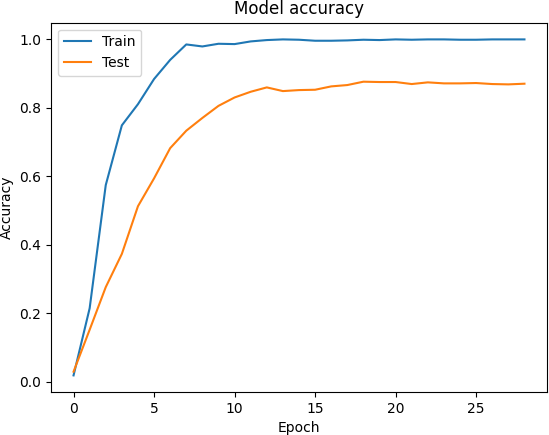
\includegraphics[width=0.48\textwidth]{images/resnet.png}} 
    \subfigure[]{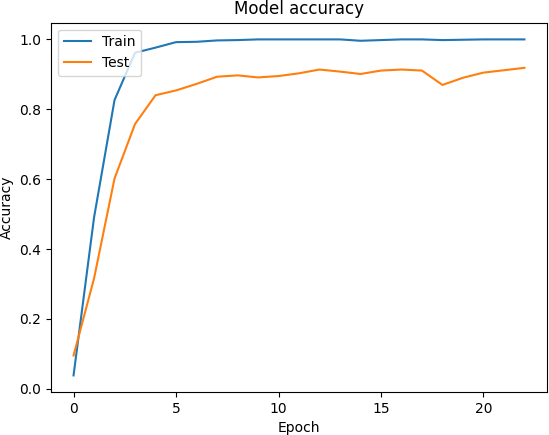
\includegraphics[width=0.48\textwidth]{images/inception.png}} 
    \subfigure[]{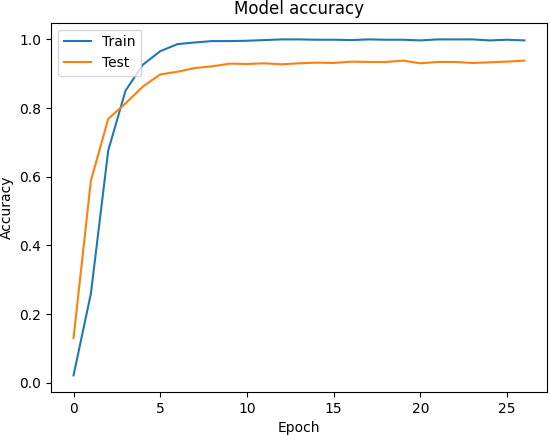
\includegraphics[width=0.48\textwidth]{images/efficient.png}} 
    \subfigure[]{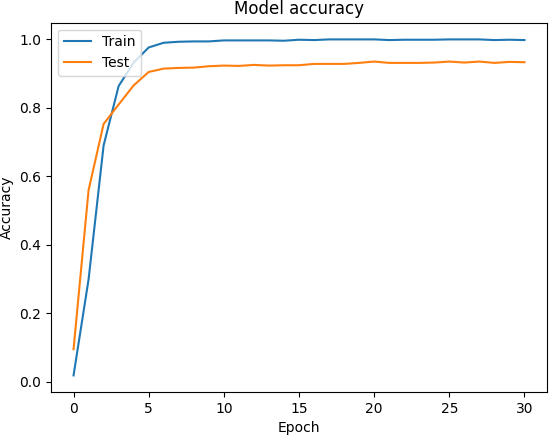
\includegraphics[width=0.48\textwidth]{images/frozen.png}} 
    \caption{Plot of the accuracy achieved by the models during the training phase: (a) \textit{ResNet-18}, (b) \textit{InceptionV3}, (c) \textit{EfficientNetB4} and (d) \textit{EfficientNetB4} with $30\%$ of untrained layers}
    \label{fig:asd}
\end{figure}


\begin{table}[ht!]
\centering
\caption{Results of the fine-tuning of \textit{ResNet-18}}
\label{tab:resnet}
\begin{tabular}{|ccll|}
\hline
\multicolumn{4}{|c|}{\textbf{ResNet-18}}                                          \\ \hline
\multicolumn{1}{|c|}{\textbf{Optimizer}}    & \multicolumn{1}{c|}{\textbf{Scheduler}}           & \multicolumn{1}{c|}{\textbf{Step size}} & \textbf{Test accuracy} \\ \hline
\multicolumn{1}{|c|}{\multirow{6}{*}{SGD}}  & \multicolumn{1}{c|}{\multirow{3}{*}{Traingular}}  & \multicolumn{1}{c|}{2}                  &  76.17\%                \\ \cline{3-4} 
\multicolumn{1}{|c|}{} & \multicolumn{1}{c|}{} & \multicolumn{1}{c|}{4} & 75.25\% \\ \cline{3-4} 
\multicolumn{1}{|c|}{} & \multicolumn{1}{c|}{} & \multicolumn{1}{c|}{8} & 75.99\% \\ \cline{2-4} 
\multicolumn{1}{|c|}{}                      & \multicolumn{1}{c|}{\multirow{3}{*}{Triangular2}} & \multicolumn{1}{c|}{2}                  &  26.52\%               \\ \cline{3-4} 
\multicolumn{1}{|c|}{} & \multicolumn{1}{c|}{} & \multicolumn{1}{c|}{4} & 50.80\% \\ \cline{3-4} 
\multicolumn{1}{|c|}{} & \multicolumn{1}{c|}{} & \multicolumn{1}{c|}{8} & 66.41\% \\ \hline
\multicolumn{1}{|c|}{\multirow{6}{*}{\textbf{Adam}}} & \multicolumn{1}{c|}{\multirow{3}{*}{\textbf{Traingular}}}  & \multicolumn{1}{c|}{\textbf{2}}                  & \textbf{87.64\%}       \\ \cline{3-4} 
\multicolumn{1}{|c|}{} & \multicolumn{1}{c|}{} & \multicolumn{1}{c|}{4} & 86.77\% \\ \cline{3-4} 
\multicolumn{1}{|c|}{} & \multicolumn{1}{c|}{} & \multicolumn{1}{c|}{8} & 85.98\% \\ \cline{2-4} 
\multicolumn{1}{|c|}{}                      & \multicolumn{1}{c|}{\multirow{3}{*}{Triangular2}} & \multicolumn{1}{c|}{2}                  & 82.48\%                \\ \cline{3-4} 
\multicolumn{1}{|c|}{} & \multicolumn{1}{c|}{} & \multicolumn{1}{c|}{4} & 84.80\% \\ \cline{3-4} 
\multicolumn{1}{|c|}{} & \multicolumn{1}{c|}{} & \multicolumn{1}{c|}{8} & 84.71\% \\ \hline
\end{tabular}
\end{table}




\begin{table}[ht!]
\centering
\caption{Results of the fine-tuning of \textit{InceptionV3}}
\label{tab:inception}
\begin{tabular}{|ccll|}
\hline
\multicolumn{4}{|c|}{\textbf{IneptionV3}}                                          \\ \hline
\multicolumn{1}{|c|}{\textbf{Optimizer}}    & \multicolumn{1}{c|}{\textbf{Scheduler}}           & \multicolumn{1}{c|}{\textbf{Step size}} & \textbf{Test accuracy} \\ \hline
\multicolumn{1}{|c|}{\multirow{6}{*}{SGD}}  & \multicolumn{1}{c|}{\multirow{3}{*}{Traingular}}  & \multicolumn{1}{c|}{2}                  &  89.98\%                \\ \cline{3-4} 
\multicolumn{1}{|c|}{} & \multicolumn{1}{c|}{} & \multicolumn{1}{c|}{4} & 89.05\% \\ \cline{3-4} 
\multicolumn{1}{|c|}{} & \multicolumn{1}{c|}{} & \multicolumn{1}{c|}{8} & 89.78\% \\ \cline{2-4} 
\multicolumn{1}{|c|}{}                      & \multicolumn{1}{c|}{\multirow{3}{*}{Triangular2}} & \multicolumn{1}{c|}{2}                  &  87.68\%               \\ \cline{3-4} 
\multicolumn{1}{|c|}{} & \multicolumn{1}{c|}{} & \multicolumn{1}{c|}{4} & 88.80\% \\ \cline{3-4} 
\multicolumn{1}{|c|}{} & \multicolumn{1}{c|}{} & \multicolumn{1}{c|}{8} & 89.66\% \\ \hline
\multicolumn{1}{|c|}{\multirow{6}{*}{\textbf{Adam}}} & \multicolumn{1}{c|}{\multirow{3}{*}{\textbf{Traingular}}}  & \multicolumn{1}{c|}{\textbf{2}}                  & \textbf{91.96\%}       \\ \cline{3-4} 
\multicolumn{1}{|c|}{} & \multicolumn{1}{c|}{} & \multicolumn{1}{c|}{4} & 91.28\% \\ \cline{3-4} 
\multicolumn{1}{|c|}{} & \multicolumn{1}{c|}{} & \multicolumn{1}{c|}{8} & 90.65\% \\ \cline{2-4} 
\multicolumn{1}{|c|}{}                      & \multicolumn{1}{c|}{\multirow{3}{*}{Triangular2}} & \multicolumn{1}{c|}{2}                  & 89.83\%                \\ \cline{3-4} 
\multicolumn{1}{|c|}{} & \multicolumn{1}{c|}{} & \multicolumn{1}{c|}{4} & 90.23\% \\ \cline{3-4} 
\multicolumn{1}{|c|}{} & \multicolumn{1}{c|}{} & \multicolumn{1}{c|}{8} & 90.79\% \\ \hline
\end{tabular}
\end{table}



\begin{table}[ht!]
\centering
\caption{Results of the fine-tuning of \textit{EfficientNetB4}}
\label{tab:efficient}
\begin{tabular}{|ccll|}
\hline
\multicolumn{4}{|c|}{\textbf{EfficientNetB4}}                                          \\ \hline
\multicolumn{1}{|c|}{\textbf{Optimizer}}    & \multicolumn{1}{c|}{\textbf{Scheduler}}           & \multicolumn{1}{c|}{\textbf{Step size}} & \textbf{Test accuracy} \\ \hline
\multicolumn{1}{|c|}{\multirow{6}{*}{SGD}}  & \multicolumn{1}{c|}{\multirow{3}{*}{Traingular}}  & \multicolumn{1}{c|}{2}                  &  91.98\%                \\ \cline{3-4} 
\multicolumn{1}{|c|}{} & \multicolumn{1}{c|}{} & \multicolumn{1}{c|}{4} & 91.74\% \\ \cline{3-4} 
\multicolumn{1}{|c|}{} & \multicolumn{1}{c|}{} & \multicolumn{1}{c|}{8} & 91.54\% \\ \cline{2-4} 
\multicolumn{1}{|c|}{}                      & \multicolumn{1}{c|}{\multirow{3}{*}{Triangular2}} & \multicolumn{1}{c|}{2}                  &  53.11\%               \\ \cline{3-4} 
\multicolumn{1}{|c|}{} & \multicolumn{1}{c|}{} & \multicolumn{1}{c|}{4} & 73.71\% \\ \cline{3-4} 
\multicolumn{1}{|c|}{} & \multicolumn{1}{c|}{} & \multicolumn{1}{c|}{8} & 86.89\% \\ \hline
\multicolumn{1}{|c|}{\multirow{6}{*}{\textbf{Adam}}} & \multicolumn{1}{c|}{\multirow{3}{*}{Traingular}}  & \multicolumn{1}{c|}{2}                  & 92.01\%       \\ \cline{3-4} 
\multicolumn{1}{|c|}{} & \multicolumn{1}{c|}{} & \multicolumn{1}{c|}{4} & 93.88\% \\ \cline{3-4} 
\multicolumn{1}{|c|}{} & \multicolumn{1}{c|}{} & \multicolumn{1}{c|}{8} & 83.37\% \\ \cline{2-4} 
\multicolumn{1}{|c|}{}                      & \multicolumn{1}{c|}{\multirow{3}{*}{\textbf{Triangular2}}} & \multicolumn{1}{c|}{2}                  & 93.93\%                \\ \cline{3-4} 
\multicolumn{1}{|c|}{} & \multicolumn{1}{c|}{} & \multicolumn{1}{c|}{\textbf{4}} & \textbf{94.89\%} \\ \cline{3-4} 
\multicolumn{1}{|c|}{} & \multicolumn{1}{c|}{} & \multicolumn{1}{c|}{8} & 92.95\% \\ \hline
\end{tabular}
\end{table}





\end{document}